\section{Introduction}
\label{sec:bcoolintro}

\begin{figure}
	\begin{center}
		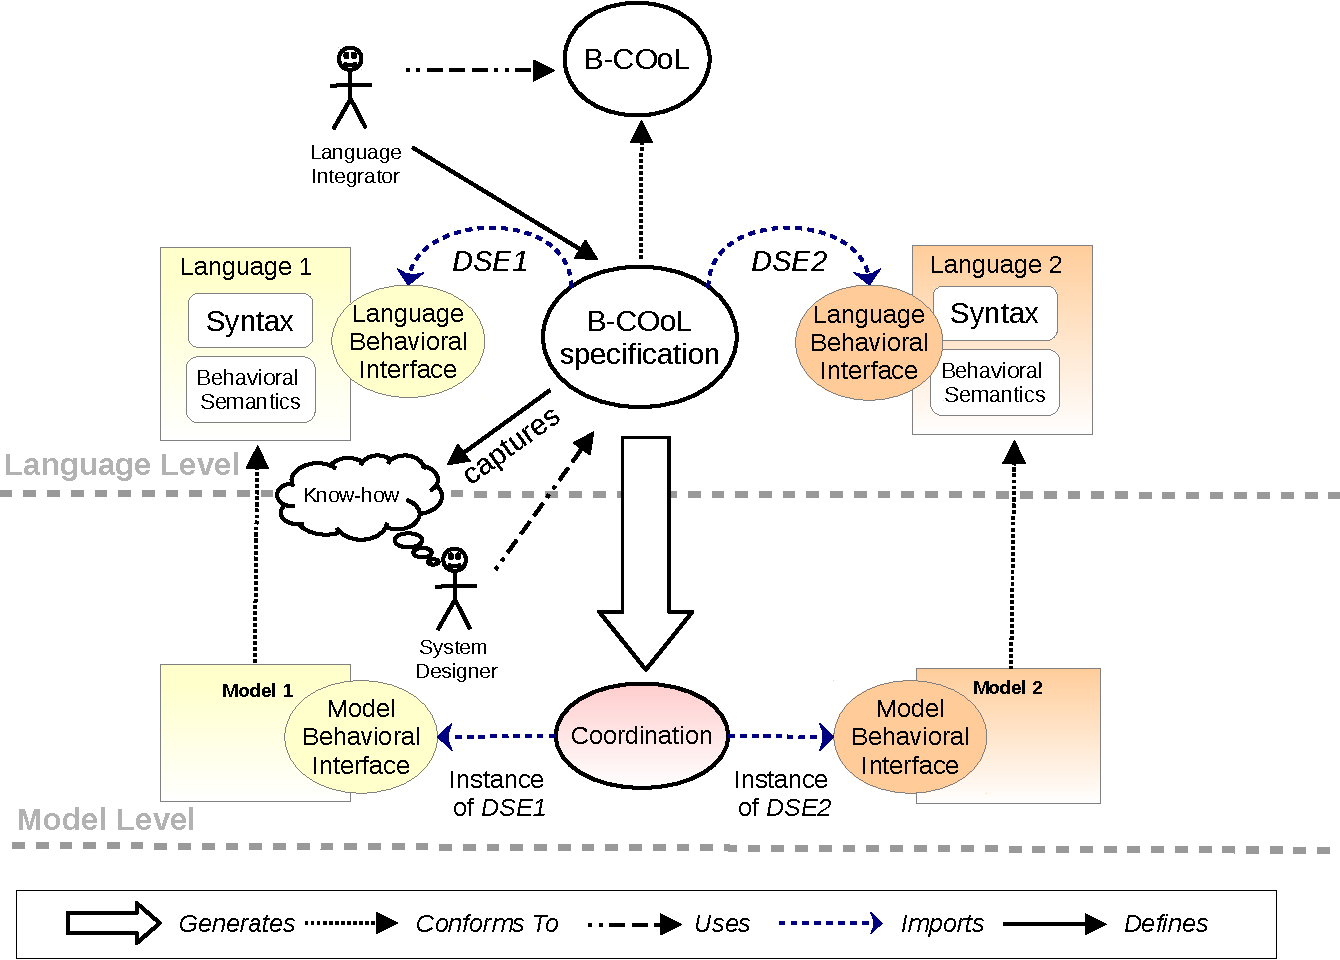
\includegraphics[width=.8\textwidth]{framework/figs/bcool}
		\caption{Overview of the Approach}
		\label{fig:bcoolapp}
	\end{center}
\end{figure}

This chapter presents \bcool, a dedicated language to specify coordination patterns. \bcool is a particular implementation of the framework presented in chapter~\ref{ch:framework}. It is based on a language behavioral interface made of event types (\ie \dse\cite{sle13-combemale}) as ``coordination points" to drive the execution of languages. These events are used as handles or control points in two complementary ways: to observe what happens inside the model, and to control what is allowed to happen or not. When required by the coordination, constraints are used to forbid or delay some event occurrences. Forbidding occurrences reduces what can be done by individual models. When several executions are allowed
(nondeterminism), it gives some freedom to individual semantics for making their own choices. All this put together makes the \dse suitable to drive coordinated simulations without being intrusive in the models. 

\bcool is a dedicated language to capture the system designer know-how (see Figure~\ref{fig:bcoolapp}). With \bcool, an \emph{language integrator} can deal with the complexity of the coordination of heterogeneous behavioral models by specifying coordination patterns at the language level. Once specified in \bcool, integrators can shared such knowledge thus allowing reusing and tuning of coordination patterns. \emph{System designers} can then use the \bcool specification to generate an explicit coordination model when specific models are used. In addition, the generated coordination model is formal thus allowing system designers to verify and validate the coordinated system.  

In \bcool, coordination patterns are captured as constraints at the language level on the \dse. A language integrator defines \emph{Operators} that are composed by a \emph{correspondence matching} and a \emph{coordination rule}. The correspondence matching identifies what elements from the behavioral interfaces (\ie what instances of \dse) must be selected. To do so, we rely on the context in which a \dse is defined to selected instances of such \dse. Then, a coordination rule specifies the, possibly timed, synchronization and causality relationships between the instances of \dse selected during the matching. To specify the coordination rule, we rely on a CCSL-based language named \moccml~\cite{moccmlbib}. The specification at language level applies between models thus generating a formal model of coordination in \ccsl.

	
%Coordination patterns are captured at language level by using operators that specify how the \dse of different language behavioral interfaces are combined and interact. Operators rely on a correspondence matching and a coordination rule. The correspondence matching identifies what elements from the behavioral interfaces (\ie what instances of \dse) must be selected. Then, a coordination rule specifies the, possibly timed, synchronizations and causality relationships between the instances of \dse selected.



In this chapter, we illustrate the use of \bcool through a simple running example: the coordination of the models of a coffee machine. To build the model, we use two languages: a state-based language named Timed Finite State Machine (TFSM) and an action-based language named Activity. The goal here is to show that we can build an operator in \bcool between these languages and then use it to coordinate the models of the coffee machine. We use this operator as running example through all the chapter. 
	
This chapter is organized as follows. We begin by introducing the running example; we show the languages, their language behavioral interfaces and the models of a coffee machine. We continue by presenting the abstract syntax and the execution semantics of \bcool. Then, we show the implementation of \bcool into the GEMOC studio. We use the studio on the running example, and we generate the coordination model for the coffee machine system. We show how the coordination model can be executed and analyzed. To finish the chapter, we compare our approach with coordination languages and frameworks, and we conclude.

%This chapter presents \bcool, a dedicated (meta)language to capture the knowledge about system integration. With \bcool, an \emph{integrator} can deal with the complexity of the coordination of heterogeneous behavioral models by capturing coordination patterns at the language level (see Figure~\ref{fig:proposedworkflow}). Coordination patterns are captured into operators that specify how \dse of different language behavioral interfaces are combined and interact. Once specified in \bcool, integrators can shared such knowledge thus allowing reusing and tuning of coordination patterns. Also, \emph{system designers} can use the \bcool specification to generate an explicit coordination model when specific models are used. Such a formal coordination model enables system designer to perform verification and validation activities on the coordinated system.     
	

%In this chapter, we illustrate the use of \bcool through a simple example: the coordination of the models of a coffee machine. To build the model, we base on two languages: a state-based language named Timed Finite State Machine (TFSM) and an action-based language named Activity. The model of the coffee machine is thus heterogeneous. We propose to coordinate these models by specifying a \bcool operator between these languages. We use this operator as running example all through the chapter. 

%\todo{This represents a typical case of separation of concern in which one domain is better described by a data-flow language and other is described by a control flow language}
%We begin this chapter by presenting the running example; we show the languages with its behavioral interface. Then, we continue by presenting our language \bcool. We illustrate it by relying on the running example. Afterward, we present the implementation of \bcool into the GEMOC studio. To finish the chapter, we evaluate and compare our approach with coordination languages and frameworks and we conclude.


%\begin{figure}
%	\begin{center}
%		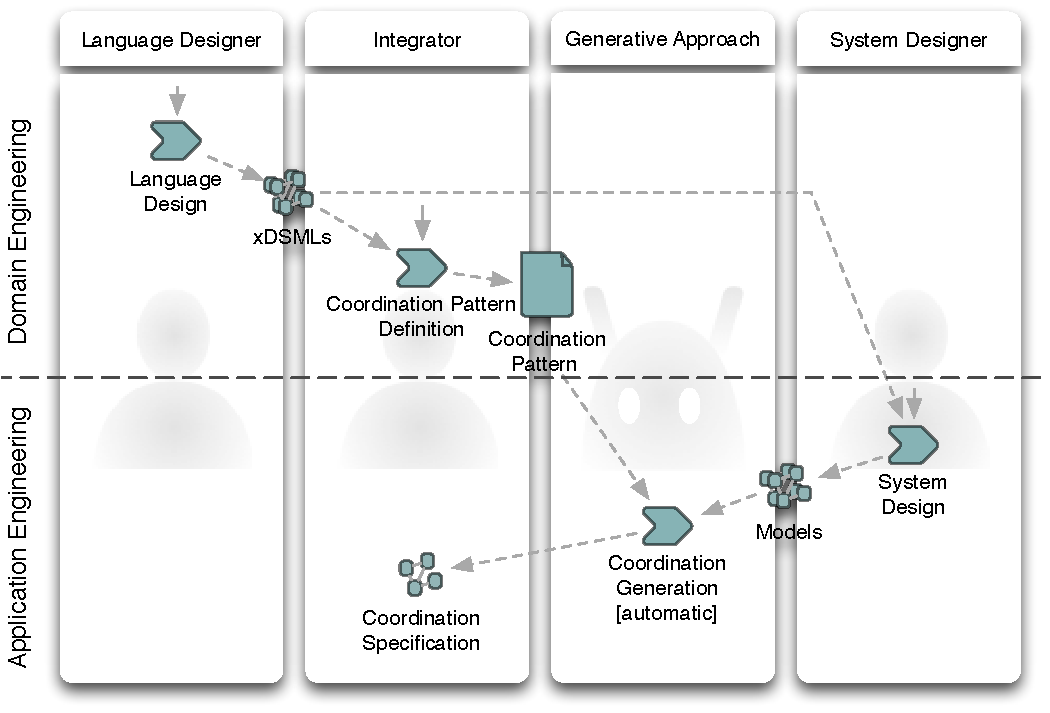
\includegraphics[width=.6\textwidth]{bcool/figs/process}
%		\caption{The Proposed Workflow}
%		\label{fig:proposedworkflow}
%	\end{center}
%\end{figure}

%The running example helps us to illustrate the different tasks in the development of heterogeneous systems:
%	\begin{enumerate}
%		\item Designing of the languages.
%		\item Integration of the languages. 
%		\item Building of the models. 
%		\item Coordination of the models. 
%	\end{enumerate}
%In this context, \bcool deal with the task number two and four. 